\chapter{Terminologies}

\begin{itemize}
	\item Le client est le commanditaire du projet.
	\item Un utilisateur est une personne souhaitant utiliser un logiciel du client. 
	\item Une licence est un droit accordé pour une machine et un utilisateur d'utiliser un logiciel donné.
	\item Craquer un logiciel est le fait de pouvoir l'utiliser sans avoir payé pour son utilisation. 
	Soit en modifiant le code compilé, soit en utilisant une autre méthode. 
\end{itemize}

\chapter{Présentation}

\chapter{Gestion de projet}

\section{Organisation}

Depuis le début du projet nous travaillons selon un fonctionnement agile, avec des
réunions et des livrables réguliers, avec le client qui se sont intensifiés au cours du semestre 2. Ce fonctionnement a permis de produire des livrables et de
la valeur rapidement.\newline

L'organisation de ce projet nous a permis de travailler efficacement, nous avions affecté un rôle à
chacun. Néanmoins, tous les acteurs de ce projet ont eu les rôles de développeur plus ou moins prononcé ainsi qu'un role de
rédacteur. Je me permet de vous renvoyer vers l'organigramme présenté dans le plan de développement en post production.\newline

Au cours de ce développement 2 Audits ont eu lieu. Cela nous a permis de comprendre les points forts mais surtout les points faibles de notre
organisation c'est pourquoi certain points ont été ajoutés/améliorés à celle-ci. \newline

Nous avons divisé la charge et la répartition par phase en méthode agile. La première phase était intitulée
«Préparation». Cette première phase a permis de donner un temps aproximatif de structuration du
projet, de vérification des répartitions des tâches et des phases de tests ce qui a donné des
évaluations de temps de développement plus précises tel que les tests de greffe de code infuctueux ou ceux
d'obfuscation. Cette phase a été suivis d'une phase de structure de projet avec le client qui a attester de la bonne évaluation de temps
et des ressources nécessaires. Après ca est venu la phase de developpement. Nous avons donc suivis une methode agile avec une période de sprint de 2 semaines, mais
celle-ci sera abordée plus en profondeur dans la prochaine section "Déroulement".\newline

\newpage

\section{Déroulement}

Le projet s'etant déroulé au cours de l'année scolaire l'organisation à du s'adapter aux
contrainte de temps de travail demandé par les autres matières ainsi qu'aux modifications d'emploie
du temps de chacun. Ce qui a donné ce diagramme de Gantt lors du second audit courant Avril.

\begin{figure}[!h]
	\centering
	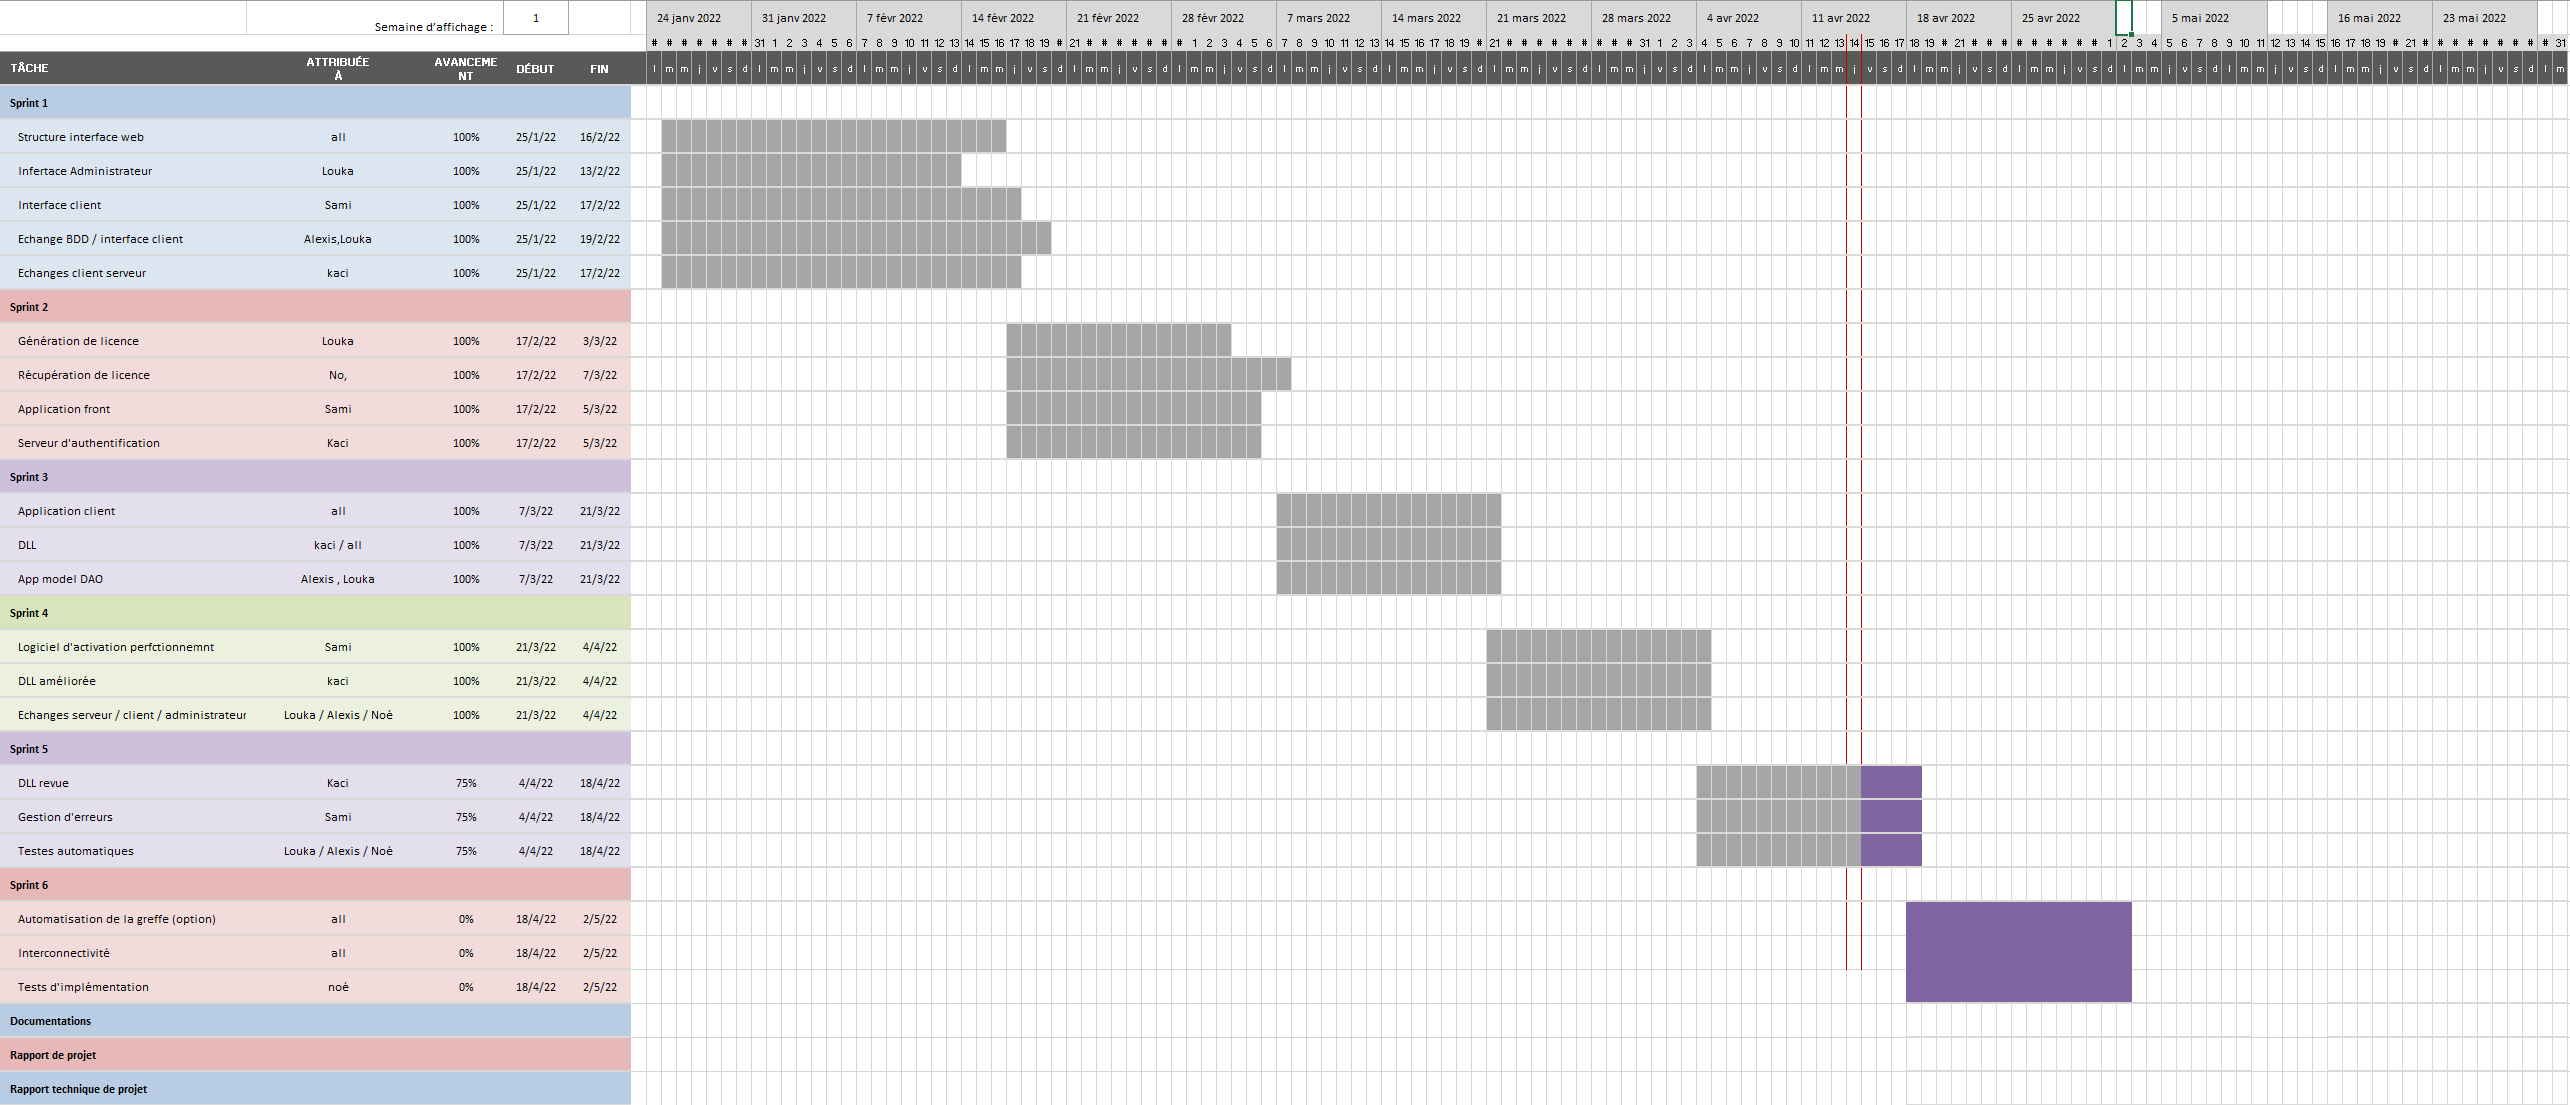
\includegraphics[width=15cm]{Gantt.png}
\end{figure}

La phase de développement du projet a donc, si nous nous referons aux anciennes estimations, suivis son cours.\newline

Celle-ci s'est donc découpé en phase de sprint de 2 semaines chacunes. Chaque sprint se décomposé de la maniere suivante :\newline  

\begin{itemize}
	\item 1 - Réunion de debut de sprint avec l'equipe pour faire une estimation de temps de taches définies ainsi que pour les attribuer.\newline
	\item 2 - Réunions journaliere pour faire le point sur les avancés et les bloquages de la veille.\newline
	\item 3 - Réalisation des taches définies.(Développement)\newline
	\item 4 - Réunion de fin de sprint (Sprint Review) avec le client pour nous donner son retour sur l'itération précédente, et démonstration faites au cours de la réunion.\newline
	\item 5 - Fin de réunion pour confirmer les prochains livrables et les dates.\newline
	\item 6 - Livraison du livrable au client.\newline
	\item 7 - Retrospective du sprint sur RetroMetro (outil de retrospective). Cet phase permet de mettre en lumiere les éléments/actions positives qui font avancer le projet ou à l'inverse ceux qui l'entrave. 
\end{itemize}

Pour avancer rapidement et efficacement, nous avons
continué d’utiliser diverses plateformes en en avons ajouté de nouvelles:\newline

\begin{itemize}
	\item Discord :\\
	Cet outil nous permet de communiquer rapidement entre nous et
    de faire des audios / visioconférences pour nos réunions. Il est aussi très utile
    pour communiquer rapidement et faire des annonces importantes (réunions,
    vérification d’un mail avant son envoi, etc.) et pour partager / archiver les
    comptes rendus de toutes les réunions.\\
	
    \item Trello :\\
	Cet outil nous permet de répartir et de savoir sur quelle tâche
    travaillent les membres de l’équipe et de connaître leur avancement.\\
		
		\item RetroMetro :\\
		Est un tableau blanc en ligne favorisant l’expression et le travail entre membres d’une même équipe 
		à distance ou même sur une même machine.Cet outil un excellent moyen de susciter toute l'equipe pour
		que tous puisse relever les bons comme les mauvais points du sprint au momment du sprint retrospective\\

    \item GitHub :\\
	L’université nous a fourni cet outil qui est très pratique pour stocker
    les documentations produites et le code source de l’application que nous
    aurons à faire lors de la phase de développement.Cette outil a aussi été utilisé pour son outil de visualisation des taches effectuées
		ce qui nous permis de créer des BurnDown Chart afin de relever les erreurs de planning ou de répartition de taches\\
	
    \item Google docs / GitHub :\\
	Ces outils nous permettent de réaliser les documents demandés
    pour la matière Gestion de Projet. Google Docs nous permet de travailler à
    plusieurs sur un même document. Les modifications apparaissent en temps
    réel et sont sauvegardées sur une période de trente jours. Il est donc possible
    de consulter des versions antérieures de nos documents en quelques clics.\\

		\item BigBlueButton :\\
		Outils de télécommunication préféré par le client pour effectuer les sprint review lors de ses déplacement.	


\end{itemize}

\chapter{Implémentation}

\section{Licence}

\section{Outils de gestion}

\section{DLL}

\chapter{Système}

\section{Machine virtuelle d'authentification}

\section{Machine virtuelle web}

\chapter{Problèmes rencontrés}

\chapter{Amélioration possible}

\section{Injection de code}

\section{Invalidation de date}

\chapter{Conclusion}
\label{chapter:bilan}

